% Kopiervorlage Vigenère-Tabelle (Tabula recta): oben Klartext, links
% Codewort-Buchstabe; jede Zeile ist das Alphabet, verschoben um ihren
% Buchstaben. Das Beispiel (Codewort FEE) passt zum Kinder-Uni-Vortrag.
% Übersetzen mit lualatex (RPTU-Hausschrift Red Hat).
\documentclass[a4paper]{article}

\usepackage{fontspec}
\setmainfont{Red Hat Text}[BoldFont={Red Hat Text SemiBold}]
\newfontfamily\display{Red Hat Display}
\usepackage[margin=1.2cm]{geometry}
\usepackage{tikz}
\pagestyle{empty}

\definecolor{darkblue}{HTML}{1F3B5B}
\definecolor{textblue}{HTML}{1F2E43}
\definecolor{orange}{HTML}{C95F25}
\definecolor{tint}{HTML}{E3EAF2}

% Buchstabe Nummer #1 (0 = A)
\newcommand{\letter}[1]{\char\numexpr 65+#1\relax}

% Beispiel: Codewort-Buchstabe F (Zeile 5), Klartext G (Spalte 6) -> L
\newcommand{\exrow}{5}
\newcommand{\excol}{6}

\begin{document}
\begin{center}

{\display\fontsize{22}{22}\selectfont\color{darkblue} VIGENÈRE-TABELLE}\par
\vspace{7mm}

% Koordinaten in Zellen; Zelle (c, r) mit c, r = 0..25 liegt bei (c+1, r+1)
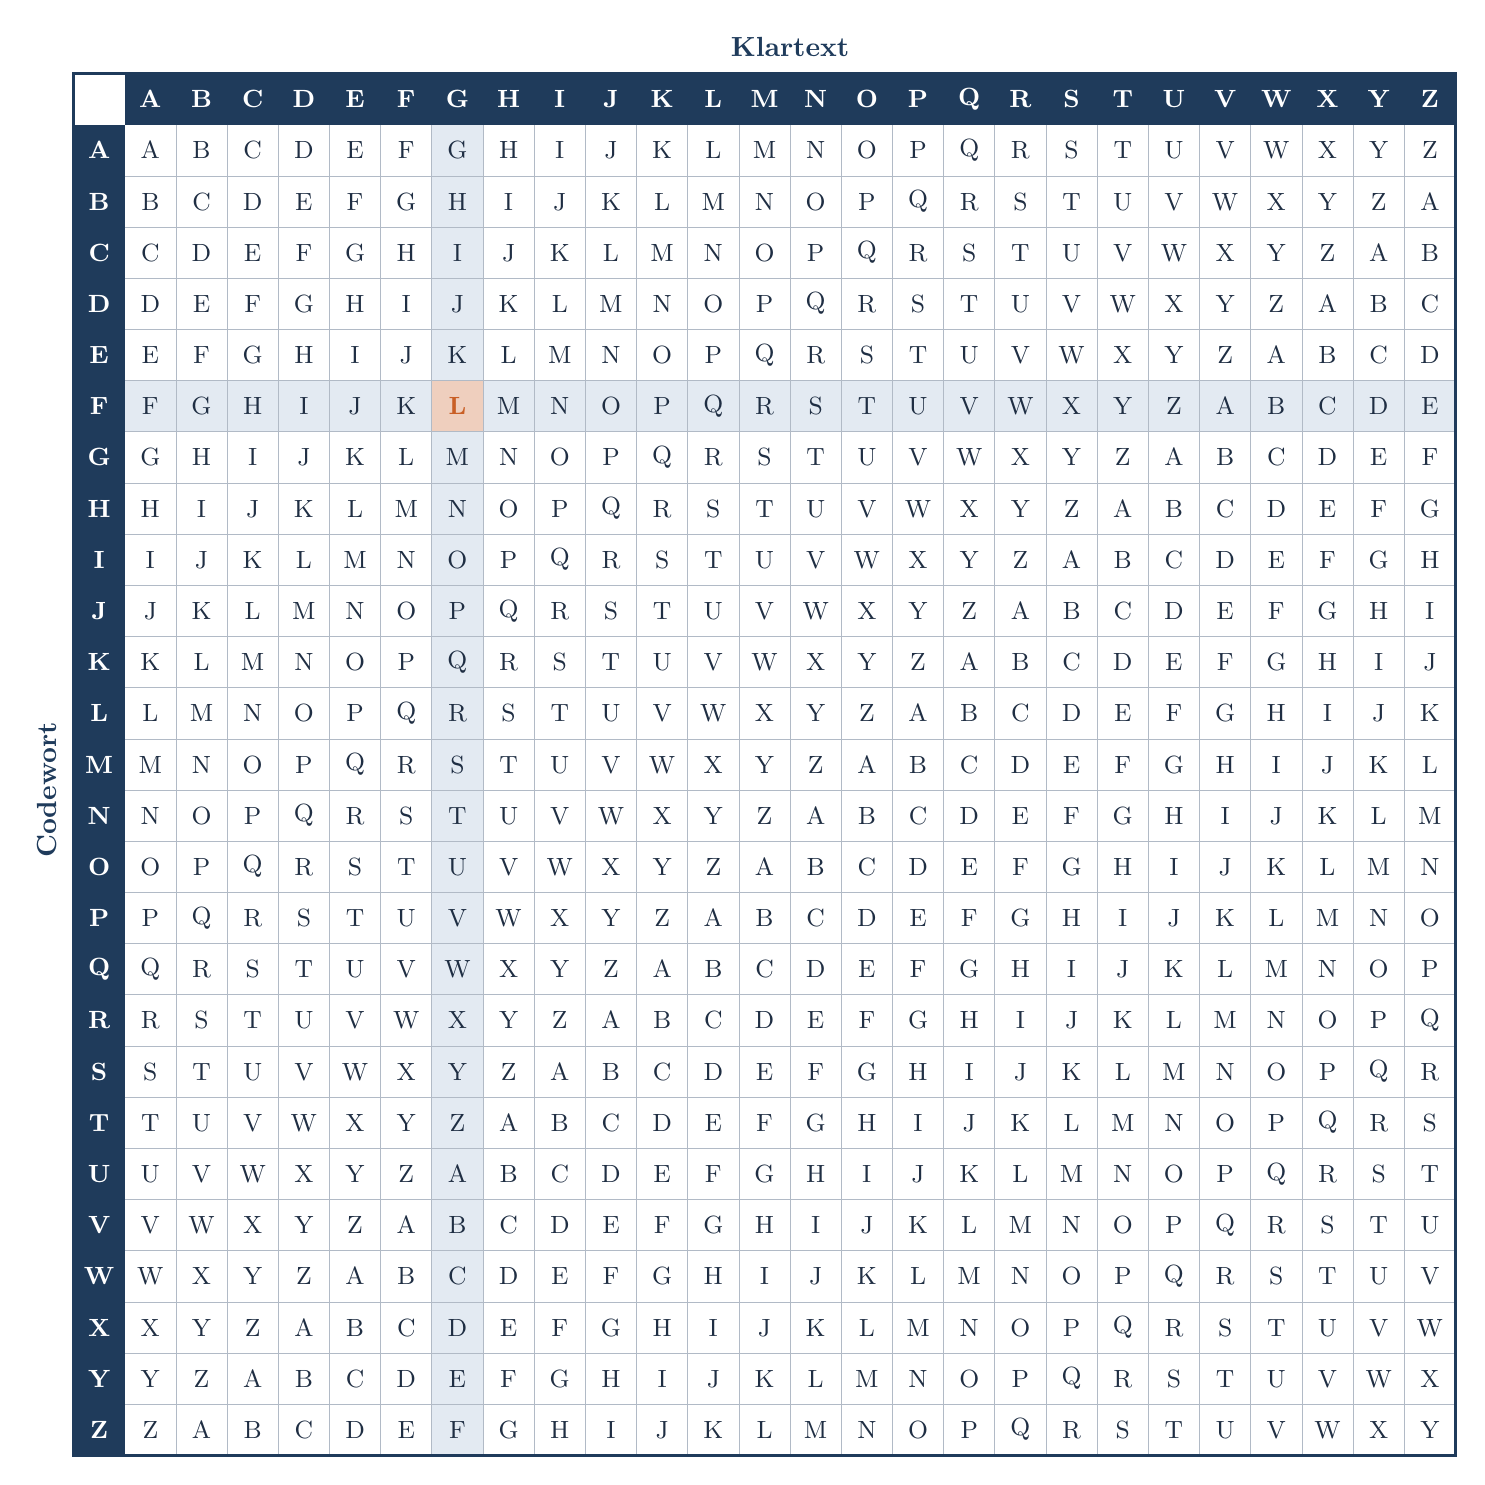
\begin{tikzpicture}[x=0.65cm, y=-0.65cm, font=\small, text=textblue]
  \fill[tint] (1, \exrow+1) rectangle (27, \exrow+2);
  \fill[tint] (\excol+1, 1) rectangle (\excol+2, 27);
  \fill[orange!30] (\excol+1, \exrow+1) rectangle (\excol+2, \exrow+2);

  \fill[darkblue] (1, 0) rectangle (27, 1);
  \fill[darkblue] (0, 1) rectangle (1, 27);
  \foreach \i in {2,...,26} {
    \draw[darkblue!35, line width=0.3pt] (\i, 1) -- (\i, 27);
    \draw[darkblue!35, line width=0.3pt] (1, \i) -- (27, \i);
  }
  \draw[darkblue, line width=1pt] (0, 0) rectangle (27, 27);

  \foreach \i in {0,...,25} {
    \node[text=white, font=\small\bfseries] at (\i+1.5, 0.5) {\letter{\i}};
    \node[text=white, font=\small\bfseries] at (0.5, \i+1.5) {\letter{\i}};
  }

  \foreach \r in {0,...,25} {
    \foreach \c in {0,...,25} {
      \pgfmathtruncatemacro{\k}{mod(\r+\c, 26)}
      \pgfmathtruncatemacro{\isex}{and(\r == \exrow, \c == \excol)}
      \ifnum\isex=1
        \node[font=\small\bfseries, text=orange] at (\c+1.5, \r+1.5) {\letter{\k}};
      \else
        \node at (\c+1.5, \r+1.5) {\letter{\k}};
      \fi
    }
  }

  \node[font=\bfseries, text=darkblue, anchor=south] at (14, -0.15)
    {Klartext};
  \node[font=\bfseries, text=darkblue, anchor=south, rotate=90] at (-0.15, 14)
    {Codewort};
\end{tikzpicture}

\vspace{6mm}

\begin{minipage}{0.92\textwidth}
  \small\color{textblue}
  \textbf{Verschlüsseln:} Schreibe das Codewort immer wieder über deine
  Botschaft. Für jeden Buchstaben suchst du oben den Klartext-Buchstaben
  und links den Codewort-Buchstaben darüber. Wo sich Spalte und Zeile
  kreuzen, steht der Geheimbuchstabe.

  \medskip
  \textbf{Beispiel:} Codewort \textbf{FEE}, Klartext \textbf{GEHEIM}.
  Spalte G und Zeile F kreuzen sich bei
  \textbf{\color{orange}L} (markiert). Insgesamt wird
  GEHEIM zu \textbf{LILJMQ}.

  \medskip
  \textbf{Entschlüsseln:} Suche in der Zeile des Codewort-Buchstabens den
  Geheimbuchstaben. Ganz oben in dieser Spalte steht der
  Klartext-Buchstabe.
\end{minipage}

\end{center}

\vfill
\begin{center}
  \scriptsize\color{textblue}
  © 2026 Max Horn, RPTU Kaiserslautern-Landau · Lizenz CC BY-SA 4.0,
  creativecommons.org/licenses/by-sa/4.0/deed.de
\end{center}
\end{document}
